\documentclass{article}

\usepackage{hyperref}
\usepackage[table]{xcolor}
\usepackage{graphicx}
\usepackage{mathtools}

\graphicspath{{images/}}

\begin{document}

\begin{titlepage}

\title{r32 CPU and Instruction Set}
\author{Reed Foster}
\date{June 2017}
\maketitle
\thispagestyle{empty}

\end{titlepage}

\pagenumbering{roman}
\tableofcontents

\newpage

\section*{About r32}
\addcontentsline{toc}{section}{About r32}
r32 is a fully-fledged, 32-bit microcontroller/SoC with a CPU-core based on the MIPS architecture.
\subsection*{Architecture}

\begin{figure}[h]
\caption{r32 Block Diagram}
\label{fig:r32blockdiagram}
\centering
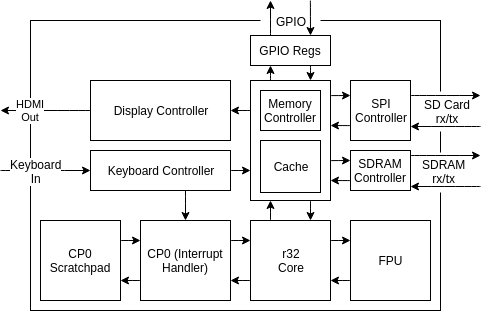
\includegraphics[scale=0.7]{architecture.png}
\end{figure}

\newpage

\pagenumbering{arabic}
\setcounter{page}{1}

\section{Instruction Set}
The r32 core instruction set is based on MIPS, an instruction set developed MIPS Technologies (founded by researchers from Stanford University). MIPS is a RISC architecture, with a 5-stage pipeline and 128-byte register file. r32's instruction set is mostly a subset of MIPS, with a few tweaks to the programmer's interface to the processor.

\subsection{Instruction Format}

Just like MIPS, r32 has three different instruction formats: r-, i-, and j-type instructions (and several other formats for floating point instructions, which are based off of r-type instructions). R-type instructions are primarily computational instructions, while i-type instructions are a mix of memory access, branch, and computation instructions, and j-type instructions are used for setting the program counter to a specific value (like an absolute branch rather than a relative one). The opcode of the instruction determines its type/format, as well as what the processor does. Registers rs and rt are source registers for r-type instructions, and rd is the destination register. For loads and stores, rs is used to determine the RAM address, while rt is either the destination or source (for load or store, respectively).

\subsubsection{R-Type Instructions}
%|opcode|rs|rt|rd|shamt|func|

\begin{tabular}[h]{l r l r l r l r l r l r}
\hline
\multicolumn{2}{| c }{opcode} & \multicolumn{2}{| c}{rs} & \multicolumn{2}{| c}{rt} & \multicolumn{2}{| c}{rd} & \multicolumn{2}{| c}{shamt} & \multicolumn{2}{| c |}{func} \\
\hline
31 & 26 & 25 & 21 & 20 & 16 & 15 & 11 & 10 & 6 & 5 & 0 \\
\end{tabular}

\subsubsection{I-Type Instructions}
%|opcode|rs|rt|imm|

\begin{tabular}[h]{l r l r l r l r}
\hline
\multicolumn{2}{| c }{opcode} & \multicolumn{2}{| c}{rs} & \multicolumn{2}{| c}{rt} & \multicolumn{2}{| c |}{imm} \\
\hline
31 & 26 & 25 & 21 & 20 & 16 & 15 & 0 \\
\end{tabular}

\subsubsection{J-Type Instructions}
%|opcode|jaddr|

\begin{tabular}[h]{l r l r}
\hline
\multicolumn{2}{| c }{opcode} & \multicolumn{2}{| c |}{jaddr} \\
\hline
31 & 26 & 25 & 0 \\
\end{tabular}

\subsection{Processor Instructions}

r32 supports a wide variety of instructions which are listed in Table \ref{tab:processorinstructions}.

\begin{table}[h]
\centering
\begin{tabular}{c c c}

\centering
\definecolor{light-gray}{gray}{0.8}
\rowcolors{1}{white}{light-gray}
\begin{tabular}[t]{| c | c | c |}
\hline
\multicolumn{3}{| c |}{CPU Core} \\
\hline
add     & addi & addiu \\
addu    & and  & andi  \\
beq     & bgez & bgtz  \\
blez    & bltz & bne   \\
j       & jr   & lb    \\
lbu     & lh   & lhu   \\
lui     & lw   & nor   \\
or      & ori  & pre   \\
sub     & sh   & sll   \\
sllv    & slt  & slti  \\
sltiu   & sltu & sra   \\
srav    & srl  & srlv  \\
sub     & subu & sw    \\
syscall & teq  & teqi  \\
tge     & tgei & tgeiu \\
tgeu    & tlt  & tlti  \\
tltiu   & tltu & tne   \\
tnei    & xor  & xori  \\
\hline
\end{tabular}

\centering
\definecolor{light-gray}{gray}{0.8}
\rowcolors{1}{white}{light-gray}
\begin{tabular}[t]{| c | c |}
\hline
\multicolumn{2}{| c |}{CP0} \\
\hline
lwc0 & mfc0 \\
mtc0 & swc0 \\
\hline
\end{tabular}

\centering
\definecolor{light-gray}{gray}{0.8}
\rowcolors{1}{white}{light-gray}
\begin{tabular}[t]{| c | c | c |}
\hline
\multicolumn{3}{| c |}{CP1 (FPU)} \\
\hline
bc1f & bc1t  & ceq  \\
cfc1 & cge   & cgt  \\
cle  & clt   & cne  \\
ctc1 & fabs  & fadd \\
fdiv & fma   & fmul \\
fneg & fsqrt & fsub \\
lwc1 & mfc1  & mov  \\
mtc1 & swc1  &      \\
\hline
\end{tabular}

\end{tabular}
\caption{Supported processor and coprocessor instructions}
\label{tab:processorinstructions}
\end{table}

\newpage

\documentclass{article}

\begin{document}

\subsection*{add}

\begin{tabular}[h]{l r l r l r l r l r l r}
\hline
\multicolumn{2}{| c }{000000} & \multicolumn{2}{| c}{rs} & \multicolumn{2}{| c}{rt} & \multicolumn{2}{| c}{rd} & \multicolumn{2}{| c}{00000} & \multicolumn{2}{| c |}{100000} \\
\hline
31 & 26 & 25 & 21 & 20 & 16 & 15 & 11 & 10 & 6 & 5 & 0 \\
\end{tabular}
\newline

Add instruction (trap on overflow)

Reg[rd] $\leftarrow$ Reg[rs] $+$ Reg[rt]

\subsection*{addi}

\begin{tabular}[h]{l r l r l r l r}
\hline
\multicolumn{2}{| c }{001000} & \multicolumn{2}{| c}{rs} & \multicolumn{2}{| c}{rt} & \multicolumn{2}{| c |}{imm} \\
\hline
31 & 26 & 25 & 21 & 20 & 16 & 15 & 0 \\
\end{tabular}

Add immediate (trap on overflow)

Reg[rt] $\leftarrow$ Reg[rs] $+$ imm$^\pm$

\subsection*{addiu}

\begin{tabular}[h]{l r l r l r l r}
\hline
\multicolumn{2}{| c }{001001} & \multicolumn{2}{| c}{rs} & \multicolumn{2}{| c}{rt} & \multicolumn{2}{| c |}{imm} \\
\hline
31 & 26 & 25 & 21 & 20 & 16 & 15 & 0 \\
\end{tabular}

Add immediate (ignore overflow, note imm is still sign extended)

Reg[rt] $\leftarrow$ Reg[rs] $+$ imm$^\pm$

\subsection*{addu}

\begin{tabular}[h]{l r l r l r l r l r l r}
\hline
\multicolumn{2}{| c }{000000} & \multicolumn{2}{| c}{rs} & \multicolumn{2}{| c}{rt} & \multicolumn{2}{| c}{rd} & \multicolumn{2}{| c}{00000} & \multicolumn{2}{| c |}{100001} \\
\hline
31 & 26 & 25 & 21 & 20 & 16 & 15 & 11 & 10 & 6 & 5 & 0 \\
\end{tabular}
\newline

Add instruction (ignore overflow)

Reg[rd] $\leftarrow$ Reg[rs] $+$ Reg[rt]

\subsection*{and}

\begin{tabular}[h]{l r l r l r l r l r l r}
\hline
\multicolumn{2}{| c }{000000} & \multicolumn{2}{| c}{rs} & \multicolumn{2}{| c}{rt} & \multicolumn{2}{| c}{rd} & \multicolumn{2}{| c}{00000} & \multicolumn{2}{| c |}{100100} \\
\hline
31 & 26 & 25 & 21 & 20 & 16 & 15 & 11 & 10 & 6 & 5 & 0 \\
\end{tabular}
\newline

Bitwise logical AND

Reg[rd] $\leftarrow$ Reg[rs] AND Reg[rt]

\subsection*{andi}

\begin{tabular}[h]{l r l r l r l r}
\hline
\multicolumn{2}{| c }{001100} & \multicolumn{2}{| c}{rs} & \multicolumn{2}{| c}{rt} & \multicolumn{2}{| c |}{imm} \\
\hline
31 & 26 & 25 & 21 & 20 & 16 & 15 & 0 \\
\end{tabular}

Bitwise logical AND with immediate

Reg[rt] $\leftarrow$ Reg[rs] AND imm$^\emptyset$

\subsection*{bc1f}

\begin{tabular}[h]{l r l r l r c c l r}
\hline
\multicolumn{2}{| c }{010001} & \multicolumn{2}{| c}{01000} & \multicolumn{2}{| c}{cc} & \multicolumn{1}{| c }{0} & \multicolumn{1}{| c }{0} & \multicolumn{2}{| c |}{imm} \\
\hline
31 & 26 & 25 & 21 & 20 & 16 & 15 & 0 \\
\end{tabular}

Branch if coprocessor 1 (FPU) false

PC $\leftarrow$ (cc = 0) ? PC $+$ offset$^\pm$ : PC $+$ 1

\subsection*{bc1t}

\begin{tabular}[h]{l r l r l r c c l r}
\hline
\multicolumn{2}{| c }{010001} & \multicolumn{2}{| c}{01000} & \multicolumn{2}{| c}{cc} & \multicolumn{1}{| c }{0} & \multicolumn{1}{| c }{1} & \multicolumn{2}{| c |}{imm} \\
\hline
31 & 26 & 25 & 21 & 20 & 16 & 15 & 0 \\
\end{tabular}

Branch if coprocessor 1 (FPU) true

PC $\leftarrow$ (cc = 1) ? PC $+$ offset$^\pm$ : PC $+$ 1

\subsection*{beq}

\begin{tabular}[h]{l r l r l r l r}
\hline
\multicolumn{2}{| c }{000100} & \multicolumn{2}{| c}{rs} & \multicolumn{2}{| c}{rt} & \multicolumn{2}{| c |}{offset} \\
\hline
31 & 26 & 25 & 21 & 20 & 16 & 15 & 0 \\
\end{tabular}

Branch if equal

PC $\leftarrow$ (rs = rt) ? PC $+$ offset$^\pm$ : PC $+$ 1

\subsection*{bgez}

\begin{tabular}[h]{l r l r l r l r}
\hline
\multicolumn{2}{| c }{000001} & \multicolumn{2}{| c}{rs} & \multicolumn{2}{| c}{0001} & \multicolumn{2}{| c |}{offset} \\
\hline
31 & 26 & 25 & 21 & 20 & 16 & 15 & 0 \\
\end{tabular}

Branch if greater than or equal to zero

PC $\leftarrow$ (rs $\geq$ 0) ? PC $+$ offset$^\pm$ : PC $+$ 1

\subsection*{bgtz}

\begin{tabular}[h]{l r l r l r l r}
\hline
\multicolumn{2}{| c }{000111} & \multicolumn{2}{| c}{rs} & \multicolumn{2}{| c}{0000} & \multicolumn{2}{| c |}{offset} \\
\hline
31 & 26 & 25 & 21 & 20 & 16 & 15 & 0 \\
\end{tabular}

Branch if greater than zero

PC $\leftarrow$ (rs $>$ 0) ? PC $+$ offset$^\pm$ : PC $+$ 1

\subsection*{blez}

\begin{tabular}[h]{l r l r l r l r}
\hline
\multicolumn{2}{| c }{000110} & \multicolumn{2}{| c}{rs} & \multicolumn{2}{| c}{0000} & \multicolumn{2}{| c |}{offset} \\
\hline
31 & 26 & 25 & 21 & 20 & 16 & 15 & 0 \\
\end{tabular}

Branch if less than or equal to zero

PC $\leftarrow$ (rs $\leq$ 0) ? PC $+$ offset$^\pm$ : PC $+$ 1

\subsection*{bltz}

\begin{tabular}[h]{l r l r l r l r}
\hline
\multicolumn{2}{| c }{000001} & \multicolumn{2}{| c}{rs} & \multicolumn{2}{| c}{0000} & \multicolumn{2}{| c |}{offset} \\
\hline
31 & 26 & 25 & 21 & 20 & 16 & 15 & 0 \\
\end{tabular}

Branch if less than zero

PC $\leftarrow$ (rs $<$ 0) ? PC $+$ offset$^\pm$ : PC $+$ 1

\subsection*{bne}

\begin{tabular}[h]{l r l r l r l r}
\hline
\multicolumn{2}{| c }{000101} & \multicolumn{2}{| c}{rs} & \multicolumn{2}{| c}{rt} & \multicolumn{2}{| c |}{offset} \\
\hline
31 & 26 & 25 & 21 & 20 & 16 & 15 & 0 \\
\end{tabular}

Branch if less not equal

PC $\leftarrow$ (rs $\neq$ rt) ? PC $+$ offset$^\pm$ : PC $+$ 1

\subsection*{ceq}

\subsection*{cfc1}

\subsection*{cge}

\subsection*{cgt}

\subsection*{cle}

\subsection*{clt}

\subsection*{cne}

\subsection*{ctc1}

\subsection*{fabs}

\subsection*{fadd}

\subsection*{fdiv}

\subsection*{fma}

\subsection*{fmul}

\subsection*{fneg}

\subsection*{fsqrt}

\subsection*{fsub}

\subsection*{j}

\subsection*{jr}

\subsection*{lb}

\subsection*{lbu}

\subsection*{lh}

\subsection*{lhu}

\subsection*{lui}

\subsection*{lw}

\subsection*{lwc0}

\subsection*{lwc1}

\subsection*{mfc0}

\subsection*{mfc1}

\subsection*{mov}

\subsection*{mtc0}

\subsection*{mtc1}

\subsection*{nor}

\subsection*{or}

\subsection*{ori}

\subsection*{pre}

\subsection*{sh}

\subsection*{sll}

\subsection*{sllv}

\subsection*{slt}

\subsection*{slti}

\subsection*{sltiu}

\subsection*{sltu}

\subsection*{sra}

\subsection*{srav}

\subsection*{srl}

\subsection*{srlv}

\subsection*{sub}

\subsection*{sub}

\subsection*{subu}

\subsection*{sw}

\subsection*{swc0}

\subsection*{swc1}

\subsection*{syscall}

\subsection*{teq}

\subsection*{teqi}

\subsection*{tge}

\subsection*{tgei}

\subsection*{tgeiu}

\subsection*{tgeu}

\subsection*{tlt}

\subsection*{tlti}

\subsection*{tltiu}

\subsection*{tltu}

\subsection*{tne}

\subsection*{tnei}

\subsection*{xor}

\subsection*{xori}

\end{document}

\newpage

\section{Memory}
Memory information

\subsection{SDRAM}
\subsubsection{What is SDRAM?}
SDRAM stands for Synchronous DRAM, or Synchronous Dynamic Random Access Memory. SRAM, or Static Random Access Memory, the fast style of memory found in cache memory on the CPU die, is made up of transistors that form a circuit that has similar behavior to a latch or flip-flop. DRAM and SDRAM, however, use small capacitors to store each bit, and as a result, DRAM-style memories are much cheaper per byte than SRAM. Because DRAM uses capacitors to store data, each bit must be refreshed frequently to maintain its state. Fortunately, SDRAM modules have control circuitry that automates a lot of the maintainance tasks surrounding DRAM, so memory controllers that interface with SDRAM aren't as difficult to design. That being said, SDRAM presents a far more complex interface than SRAM. One of the first confusing things for beginners is how SDRAM can have millions of addresses, despite a 12- or 13-bit address ($2^{13} = 8192$ or $8K$). In order to access a word of data in SDRAM, one must first activate a row in a bank, and then supply a column address to access a byte when reading. This essentially doubles the 12 or 13 bits of address, allowing for the user to access millions of separate addresses. One of the neat things about SDRAM that allows it to perform very well despite large latencies (which increase at higher clock frequencies) is its capability to burst. The particular SDRAM on the minispartan6+ development board used to develop the r32 allows for 1-word, 2-word, 4-word, 8-word, and full-page (512-word) bursts. Because the r32 specifies a caching hierarchy, the memory controller uses a 512-word burst to maximize bandwith. By only reading or writing to RAM when a cache miss occurs, the controller logic is greatly simplified.

\subsubsection{Finite State Machine}
At the heart of the SDRAM controller is a Finite State Machine, or FSM. Figure \ref{fig:sdramfsm} shows the 2nd (current) revision of the SDRAM state machine used to drive the controller. The green states indicate states in which data is being transferred (read/written). First, the SDRAM is initialized (blue states). The datasheet for the SDRAM chip specifies a 200$\mu$s startup where all control signals must be held constant. This is achieved by using a counter that counts from $200,000 / t_{ck}$ to 0 where $t_{ck}$ is the period of the clock (ns). The rest of the delays are implemented the same way. The loopback state transitions labeled $t_{rp}$, $t_{mrd}$, $t_{rp}$, etc. are timing constraints specified in the SDRAM datasheet.

\begin{figure}[!htb]
\caption{SDRAM Finite State Machine}
\label{fig:sdramfsm}
\centering
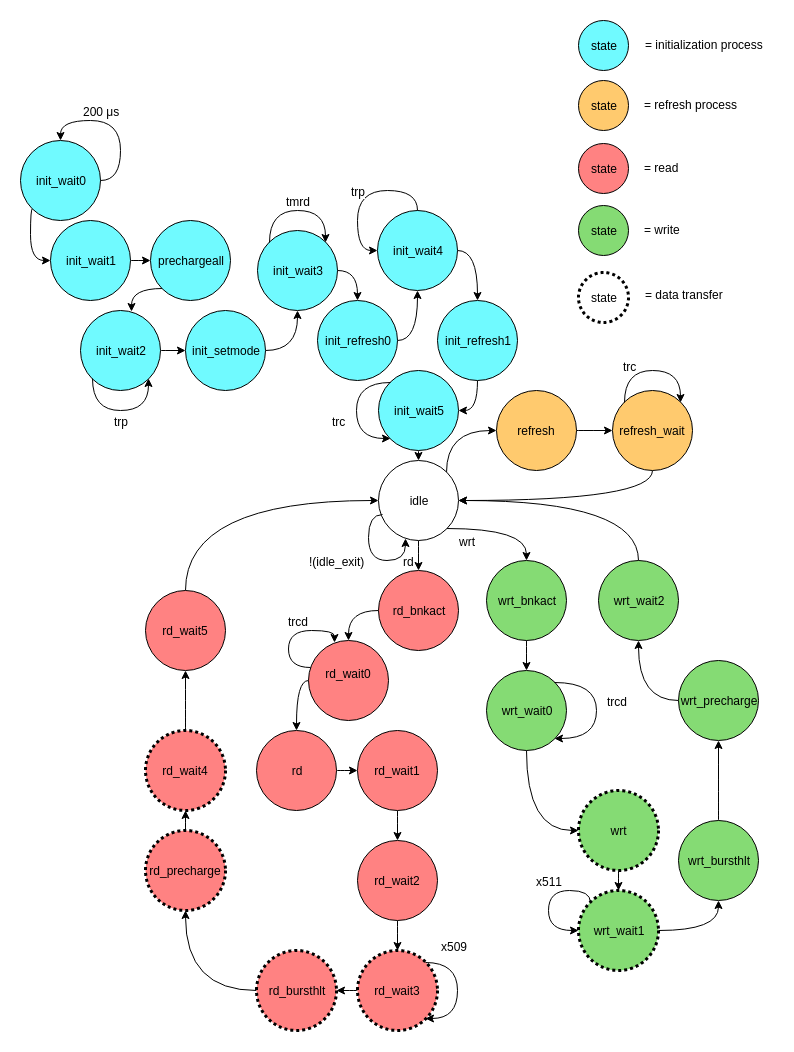
\includegraphics[scale=0.23]{sdramfsm2.png}
\end{figure}

\newpage

\subsubsection{FIFOs}
In order to maximize cache efficiency, I have added FIFO queues to the data input and output on the SDRAM controller. This allows the cache to quickly free up a line that has old data in it by writing the evicted data to a buffer without waiting for the controller to be ready to write. The FIFO on the output of the controller achieves a similar goal, alllowing the SDRAM controller to read from the SDRAM uninterrupted and write all of the read data to the buffer. In addition to buffering data, I also use a small FIFO as a "request" queue. This allows the CPU cache logic to make requests to read or write to SDRAM, even if the SDRAM controller is currently accessing the SDRAM. The CPU cache can request to write data and begin to write data into the transmit FIFO while the SDRAM controller is still busy processing a previous read or write request, and then proceed to manage the cache until it the data is ready. Originally, all FIFO queues were synchronous, with a single clock for both enqueue and dequeue operations. However, I decided that in order to test that the burst was working properly, I should add dual-clock or asynchronous FIFOs so that I can read data out very slowly (i.e. a human can see the contents of each memory location with 8 leds) from the data out queue.

\newpage

\section{I/O}
I/O information
\end{document}